\begin{frame}
  \titlepage
\end{frame}

\begin{frame}
  \centering
  \begin{figure}
    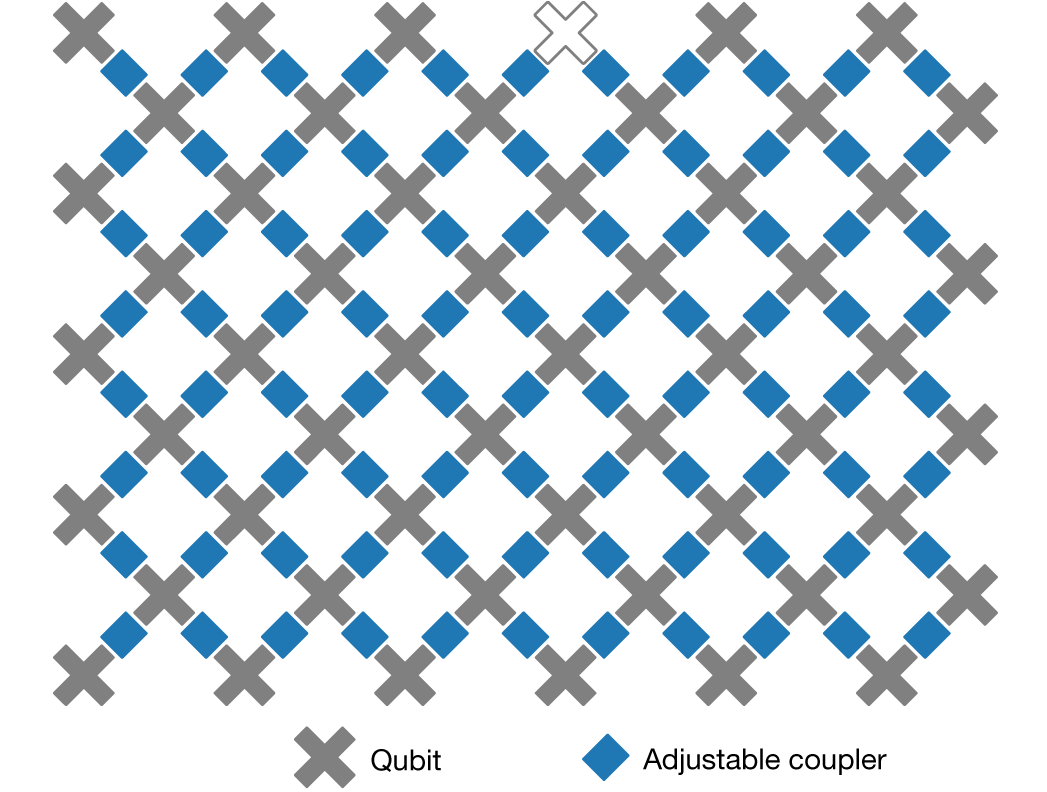
\includegraphics[width=0.6\textwidth]{figs/sycamore_precessor.png}
  \end{figure}
  {\small \color{spingrey} Arute et al. Nature 574, 505–510 (2019)}
\end{frame}

\begin{frame}
  \centering
  \begin{figure}
    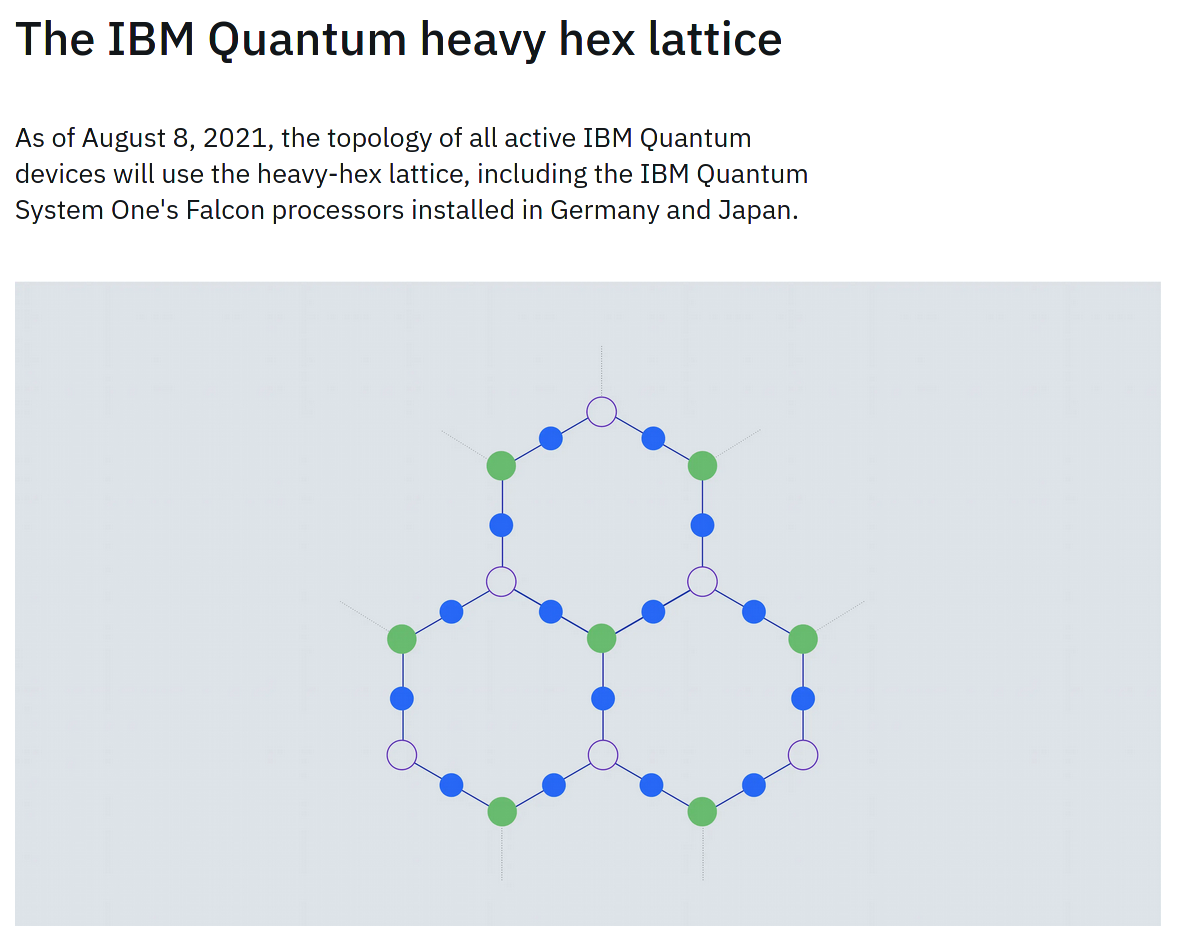
\includegraphics[width=0.7\textwidth]{figs/ibm_lattice.png}
  \end{figure}
\end{frame}

\begin{frame}
  \centering
  \Huge 
  \color{spinprimary}
  Near-term quantum computers will be locally connected.
\end{frame}

\begin{frame}
  \centering
  \begin{figure}
    
\includegraphics[width=0.2\textwidth]{figs/microsoft.png}
  \end{figure}
  \LARGE
  Can we achieve large scale fault-tolerant quantum computing on locally connected devices?
\end{frame}

\begin{frame}[c]
  \centering
  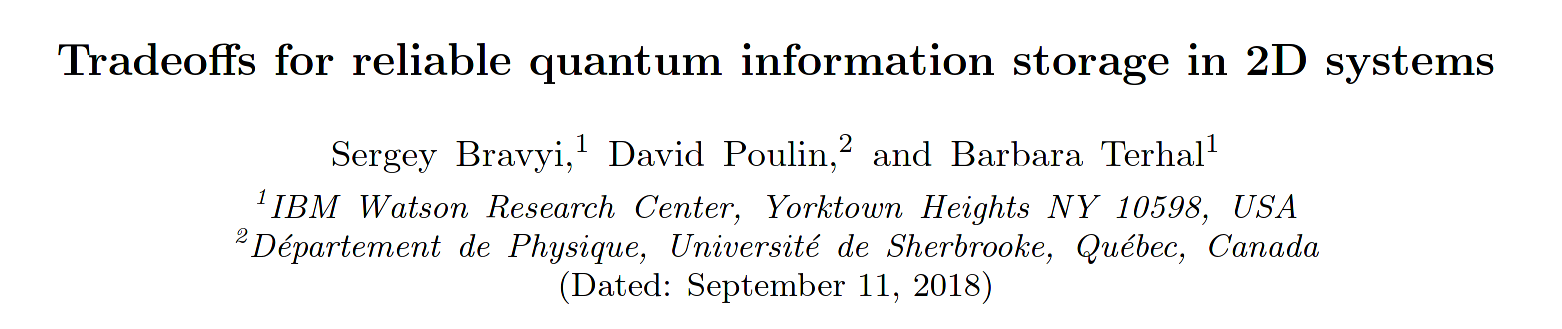
\includegraphics[width=\textwidth]{figs/bpt.png}
\end{frame}

\begin{frame}[c]{Long range interactions from local operations}
  \centering
  \hfill\\[1cm]
  \pause
  \begin{tikzpicture}  
    \draw[line width=0.75mm] (0,0) -- (5,0);
    \draw[line width=0.75mm] (7,0) -- (12,0);
    \draw[line width=0.75mm] (5.4,0) -- (5.6,0);
    \draw[line width=0.75mm] (5.9,0) -- (6.1,0);
    \draw[line width=0.75mm] (6.4,0) -- (6.6,0);

    \fill[spinprimary] (0,0) circle (0.4);
    \fill[spinsecondary] (2,0) circle (0.4);
    \fill[spinsecondary] (4,0) circle (0.4);
    \fill[spinsecondary] (8,0) circle (0.4);
    \fill[spinsecondary] (10,0) circle (0.4);
    \fill[spinprimary] (12,0) circle (0.4);
   
    \draw 
      [decorate, decoration = {calligraphic brace, amplitude=10pt}, line width=0.75mm] 
      (11, -0.75) --  (1, -0.75);

    \node (cat) at (6, -1.75) {\Large $\ket{\bar{0}} \equiv \ket{++\cdots++} + \ket{--\cdots--}$};
  \end{tikzpicture}
  \hfill\\
  \pause
  \begin{equation*}
    \Qcircuit @C=2em @R=2em {
      \lstick{} & \ctrl{2} & \qw      & \qw \\
      \lstick{} & \qw      & \ctrl{1} & \qw
      \inputgroupv{1}{2}{1em}{1em}{\color{spinprimary}\boldsymbol{\ket{\psi}}} \\
      \lstick{\color{spinsecondary}\boldsymbol{\ket{\bar 0}}} 
      & \targ & \targ & \gate{M_{\bar Z}}
    }
  \end{equation*}
\end{frame}

\begin{frame}[c]{Long range interactions from local operations}
  \centering
  \begin{equation*}
  \Qcircuit @C=1.25em @R=1.25em { 
    \lstick{\ket{0}} & \multigate{2}{M_{XX}} & \qw       & \qw                   & \qw              & \qw \\ 
    \lstick{0}       & \cghost{M_{XX}}       & \cctrl{1} &                       &                  &     \\ 
    \lstick{\ket{0}} & \ghost{M_{XX}}        & \gate{Z}  & \multigate{2}{M_{XX}} & \qw              & \qw \\ 
    \lstick{0} & \cw & \cw & \cghost{M_{XX}} & \cctrl{1} &                       &                  &     & & & \ket{++++} + \ket{----} \\ 
    \lstick{\ket{0}} & \multigate{2}{M_{XX}} & \qw       & \ghost{M_{XX}}        & \gate{Z} \cwx[2] & \qw \\ 
    \lstick{0}       & \cghost{M_{XX}}       & \cctrl{1} &                       &                  &     \\ 
    \lstick{\ket{0}} & \ghost{M_{XX}}        & \gate{Z}  & \qw                   & \gate{Z}         & \qw  
    \gategroup{1}{6}{7}{6}{1.25em}{\}}
  }
  \end{equation*}
\end{frame}

\begin{frame}[c]{Long range interactions from local operations}
  \centering
  \begin{equation*}
  \Qcircuit @C=1.25em @R=1.25em { 
    \lstick{\ket{\psi_1}} & \qw                   & \qw       & \qw                   & \qw              & \qw & \ctrl{1}  & \qw & \qw        & \qw \\ 
    \lstick{\ket{0}}      & \multigate{2}{M_{XX}} & \qw       & \qw                   & \qw              & \qw & \targ     & \qw & \gate{M_Z} \\ 
    \lstick{0}            & \cghost{M_{XX}}       & \cctrl{1} &                       &                  &     &           &     &     \\ 
    \lstick{\ket{0}}      & \ghost{M_{XX}}        & \gate{Z}  & \multigate{2}{M_{XX}} & \qw              & \qw & \qw       & \qw & \gate{M_Z} \\ 
    \lstick{0}            & \cw                   & \cw       & \cghost{M_{XX}}       & \cctrl{1}        &     &           &     &      &  & \text{parity} \\ 
    \lstick{\ket{0}}      & \multigate{2}{M_{XX}} & \qw       & \ghost{M_{XX}}        & \gate{Z} \cwx[2] & \qw & \qw       & \qw & \gate{M_Z} \\ 
    \lstick{0}            & \cghost{M_{XX}}       & \cctrl{1} &                       &                  &     &           &     &     \\ 
    \lstick{\ket{0}}      & \ghost{M_{XX}}        & \gate{Z}  & \qw                   & \gate{Z}         & \qw & \targ     & \qw & \gate{M_Z} \\ 
    \lstick{\ket{\psi_2}} & \qw                   & \qw       & \qw                   & \qw              & \qw & \ctrl{-1} & \qw & \qw        & \qw
    \gategroup{2}{8}{8}{9}{1em}{\}}
  }
  \end{equation*}
\end{frame}

\begin{frame}{Main results}
  \centering
  \hfill\\
  \begin{theorem}
    Let $C$ be a Clifford circuit measuring computing Pauli operators $S_1, \ldots, S_r$.
    Then, for any subset of qubits $L$, we have
    \begin{equation*}
      \text{depth}(C) 
      \geq
      \frac
        {n_{\text{cut}}}
        {64 |\partial L|}.
    \end{equation*}
  \end{theorem}
  \pause
  \begin{corollary}
    For families of local-expander quantum LDPC codes of length $n$,
    a syndrome extraction circuit $C$ implemented as a local Clifford circuit 
    on a $\sqrt{N} \times \sqrt{N}$ grid of qubits
    satisfies
    \begin{equation*}
      \text{depth}(C) 
      \geq
      \Omega \left(
        \frac 
          {n}
          {\sqrt{N}}
      \right).
    \end{equation*}
  \end{corollary}
\end{frame}

\begin{frame}
  \centering
  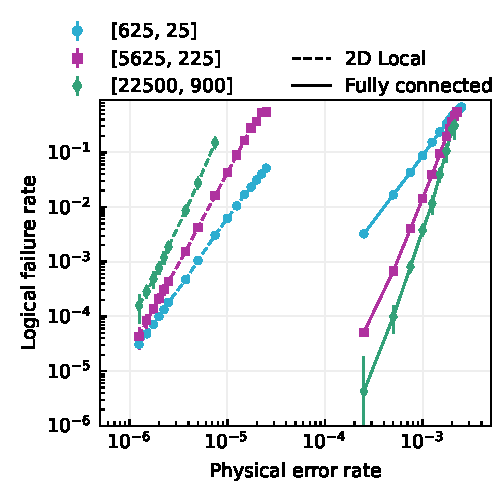
\includegraphics{figs/comparison_alt.pdf}
\end{frame}

\begin{frame}{References}
  \begin{itemize}
    \item 
      Bounds on stabilizer measurement circuits and obstructions to
      local implementations of quantum LDPC codes \\
      {\color{spinsecondary}\textbf{arXiv}} 2109.14599
    \item 
      Constant-overhead quantum error correction with thin planar connectivity \\
      {\color{spinsecondary}\textbf{arXiv}} 2109.14609
  \end{itemize}
\end{frame}

\begin{frame}{Outline}
  \begin{enumerate}
    \item Background and definitions
    \item Proof of the main theorem
    \item Circuit implementations
    \item Numerical experiments
  \end{enumerate}
\end{frame}
